\documentclass[a4paper,11pt]{article}

\usepackage[utf8]{inputenc}

\usepackage{graphicx}
\usepackage{caption}
\usepackage{subcaption}

\usepackage{pgfplots}
\pgfplotsset{compat=1.18} 

\usepackage{comment}

\usepackage{gensymb}

\begin{document}

\title{
  \textbf{Mean Sea Level Pressure} \\
  a look at some atmospheric data
}
\author{Johan Montelius}
\date{\today}

\maketitle

\section*{Introduction}

The mean sea level pressure is a calculated pressure of what it would
be if the pressure was measured at sea level. If we have measuring
stations close to the sea, the value is what is measured but if we have
data from higher grounds we need to convert the measured values to the
sea level equivalent.

In this report we will examine changes in the mean sea level pressure
around the globe during the last fifty years. The statistical
computations have been performed in Python using several statistical
libraries. Jupyter has been the development framework and ChatGPT has
been used to generate much of the code.

\subsection*{the data}

The data is "Monthly NCEP/DOE Reanalysis 2", obtained from the
National Centers for Environmental Prediction, and consists of the
monthly values from January 1979 to December 2025. A grid of $2.5
\degree \times 2.5 \degree$ squares have been modeled from various
data sources. This would give us $72 \times 144 = 10 368$ grid cells
but the data contains $73$ latitude values including both
$90\degree$ and $-90\degree$; it is not clear how this should be
interpreted.

We have time series of a total of $47$ years or $564$ months and the
mean sea level pressure varies from $960\; hPa$ to $1060\; hPa$.
 
It should be noted that a $2.5 \degree \times 2.5 \degree$ sector is
quite large. At the equator it is a square of aprx. $280 \; km \times
280\; km$. Closer to the poles the north-south distance remains the
same but the east-west distance decrease; In Sweden the sector has an
approximately east-west extension of $140\; km$.

The data that we have is a compilation of data from different
sources. These measurements are combined to give an estimate of the air
pressure in each sector around the globe. This means that a value for
a sector could be the average from more than one measuring station in
the sector or a value calculated from measuring stations outside of
the sector. This is important to realize when we later interpret our
statistical findings. 

\subsection*{one sector}

To get a better understanding of what the air pressure looks like over
time we can take a look at the data we have for the grid covering
Stockholm ($lat\; 57.5\degree \; lon\; 17.5\degree\; +
2.5\degree$). As seen in Fig.\ref{fig:stockholm}, the monthly mean
values vary quite a lot with no apparent pattern. The average value is
$1013\; hPa$ which, not surprising, is the standardized mean sea level air
pressure. The difference from the mean show a close correlation to a natural
distribution with $\sigma = 473\; Pa$; it is almost symmetrical with a
standardized skewness of $-0.046$ but slightly heavy tailed with a {\em Pearson
kurtosis} of $3.7$.

\begin{figure}[t]
  \centering
  \hspace*{-2cm}
  \begin{subfigure}{.5\paperwidth}
    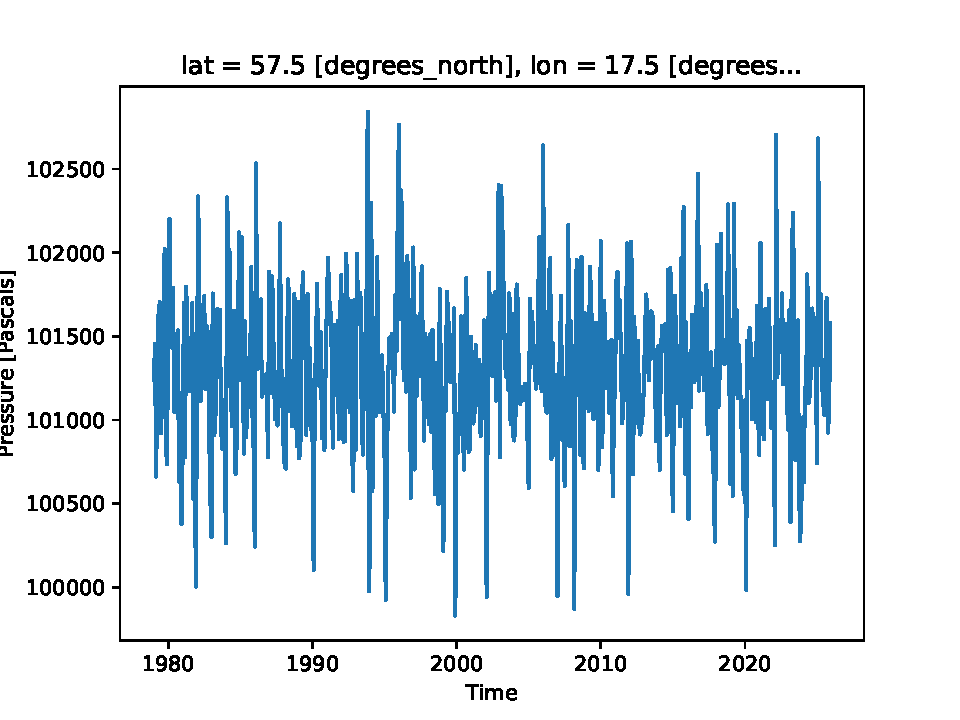
\includegraphics[scale=0.5]{stockholm-full.pdf}
    \caption{Montly mean values}
  \end{subfigure}%
  \begin{subfigure}{.5\paperwidth}
    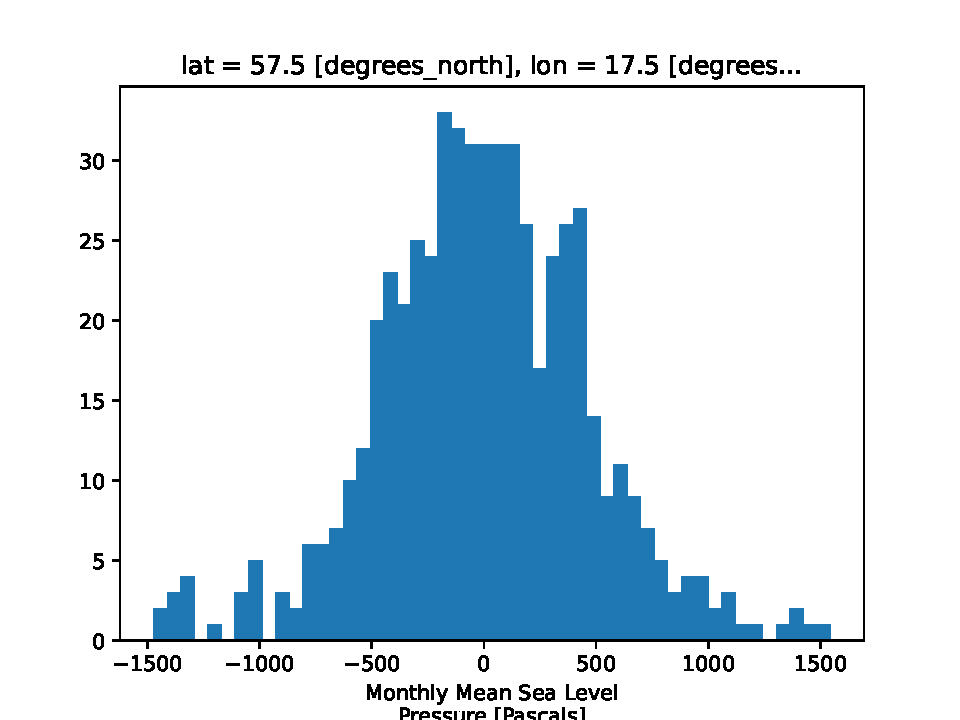
\includegraphics[scale=0.5]{stockholm-hist.pdf}
    \caption{Difference from mean.}
  \end{subfigure}
  \caption{The grid covering Stockholm.}
  \label{fig:stockholm}
\end{figure}

Since this sector is a quite populated area with several meteorological
stations we could consider these values to be fairly accurate. When we
look at sectors in the middle of Siberia, the Pacific Ocean or Antarctica -
we should take the data with a grain of salt.

\section*{Task I - changes between first and second period}

As one can see in Fig.\ref{fig:mean-global} the mean pressure over the time
period does vary over the globe. We have a band of low pressure
between $50 \degree$ and $75\degree$ south. Higher pressure is found
north and south of the tropic of Cancer and Capricorn respectively. 
 
\begin{figure}[ht!]
  \centering
  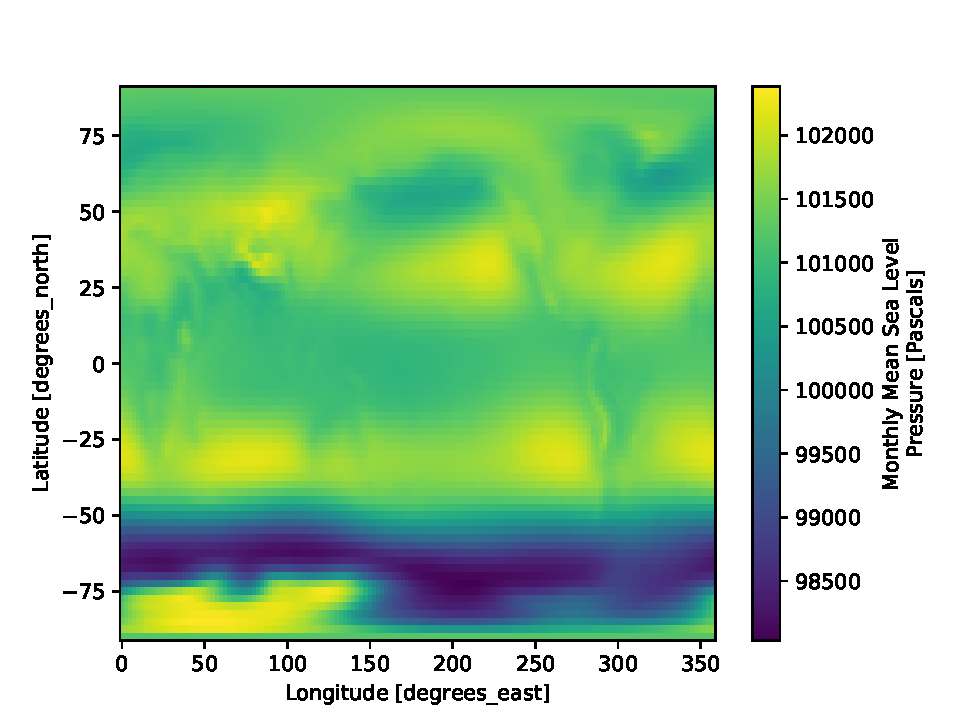
\includegraphics[width=0.4\paperwidth]{mean-global.pdf}
  \caption{Mean sea level pressure for the whole period.}
  \label{fig:mean-global}
\end{figure}

If we plot the data on a globe, as in Fig \ref{fig:mean-hemi}, we
clearly see how the low pressure surrounds Antarctica and how the high
pressure lies over the Atlantic, Pacific and Indian Ocean.

\begin{figure}[ht!]
  \centering
  \hspace*{-4cm}
  \begin{subfigure}{.4\paperwidth}
    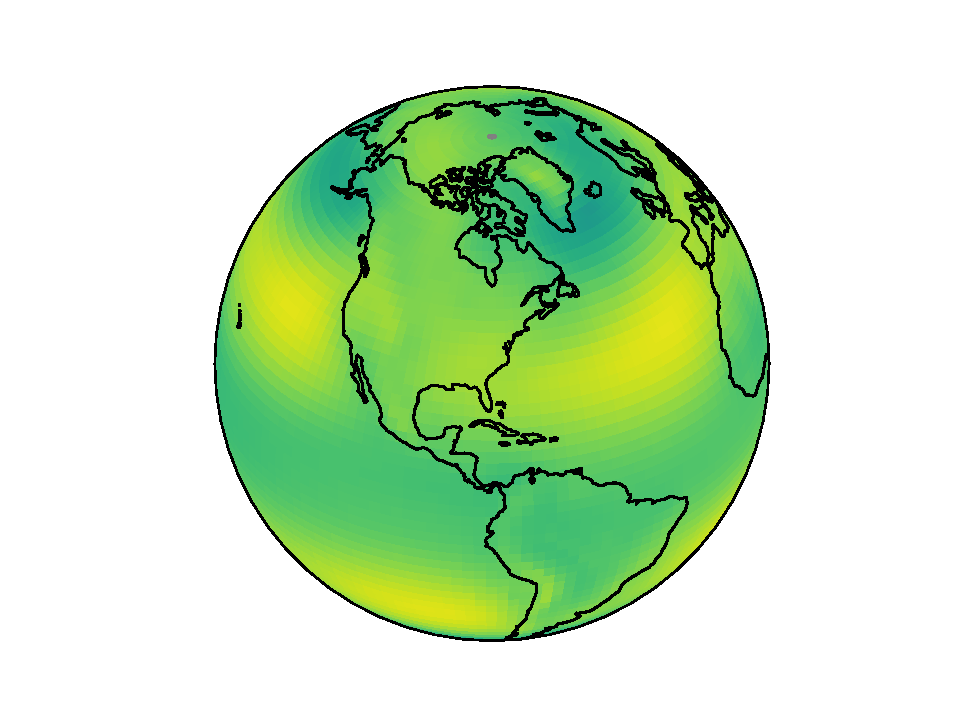
\includegraphics[scale=0.6]{mean-north.pdf}
    \caption{Northern hemisphere}
  \end{subfigure}%
  \begin{subfigure}{.6\paperwidth}
    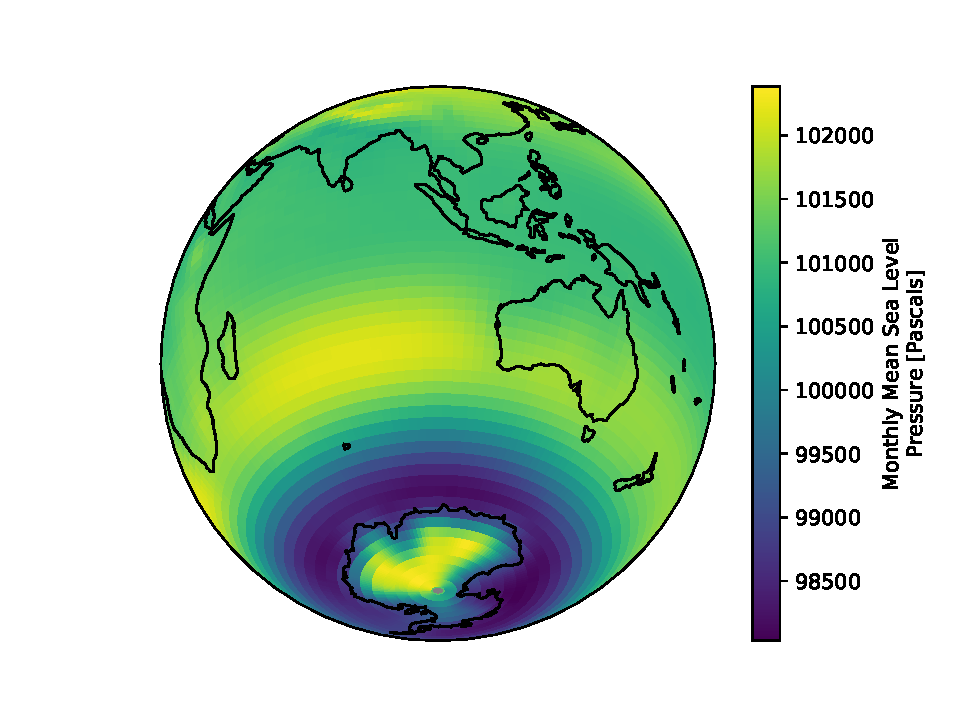
\includegraphics[scale=0.6]{mean-south.pdf}
    \caption{Southern hemisphere.}
  \end{subfigure}
  \caption{The low pressure clearly suround Antarctica. }
  \label{fig:mean-hemi}
\end{figure}

\begin{comment}

Calculate the climatologies for the first and second halves of the
record (at each grid point).  Analyse the difference between these
climatologies and its significance (can take α = 5%).  Plot a map of
the difference (second half minus first half) and the result of the
significance.

\end{comment}

If we divide the time series in two segments we can compare the first
part of the time series with the second. The difference in mean sea
level air pressure is shown in Fig.\ref{fig:dif-global}. The data shows a
difference in the Pacific just north of Antarctica where the mean sea
level air pressure has decreased by about $200-300\; Pa$. North of
this region we see an increase over the Pacific by about $100-200\;
Pa$. In the northern hemisphere there is a slight decrease apart from
two outliers, one on Greenland and the other around the Caspian sea.

The measurements at any given location can vary by $10\; hPa$ between
a high and low pressure so a change of $0.2\; hPa$ is quite small in
comparison. The standard deviation in the Stockholm segment was aprx
$0.5\; hPa$ so we are looking at changes that are less than half a
standard deviation.

\begin{figure}[ht!]
  \centering
  \hspace*{-4cm}
  \begin{subfigure}{.4\paperwidth}
    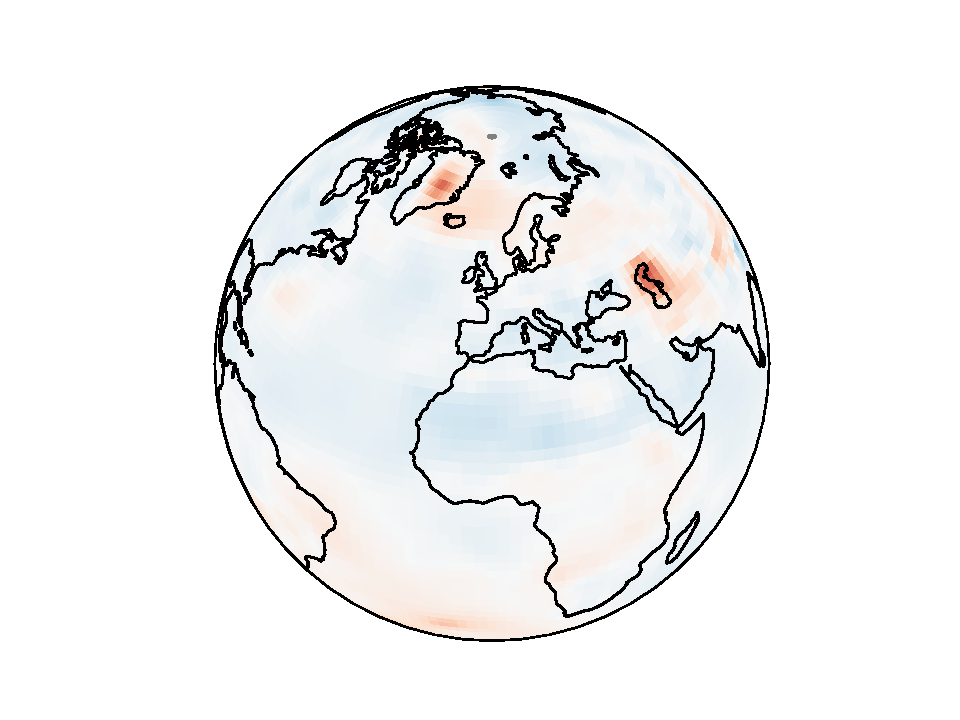
\includegraphics[scale=0.6]{dif-north.pdf}
    \caption{Northern hemisphere}
  \end{subfigure}%
  \begin{subfigure}{.6\paperwidth}
    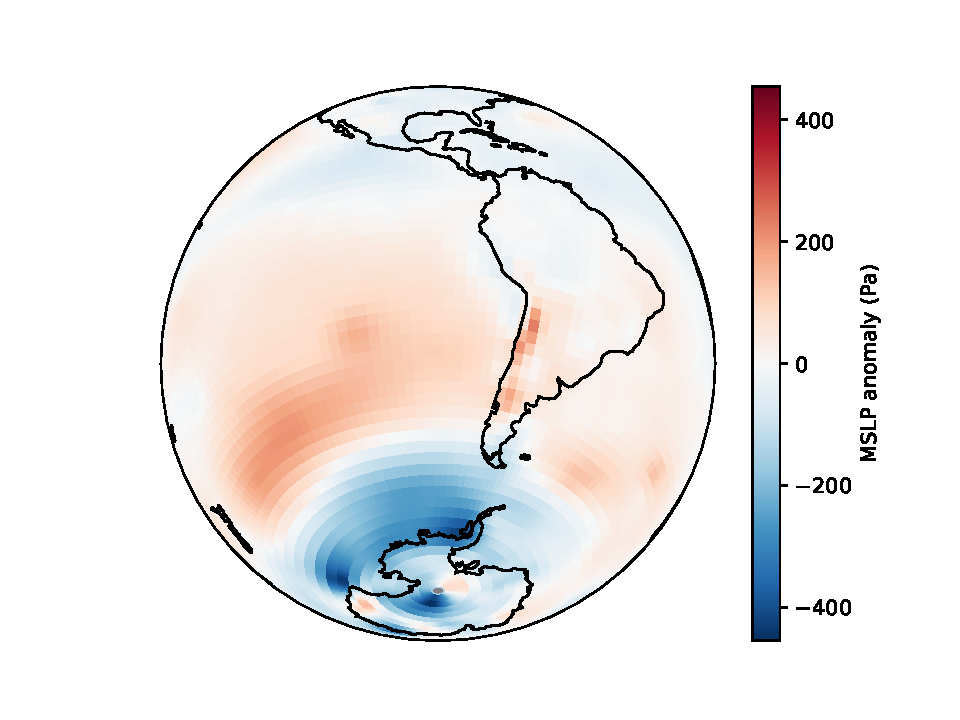
\includegraphics[scale=0.6]{dif-south.pdf}
    \caption{Southern hemisphere.}
  \end{subfigure}
  \caption{Difference of mean between first and second half of the time series. } 
  \label{fig:dif-global}
\end{figure}


We also must consider that the data we have is not directly measured
valued but values extrapolated from various sources: fixed stations,
balloons, ships, satellites etc. What are the data that we have for
Antarctica built from? Is the values in the south Pacific just the
average of a station at Pitcairn Island and the McMurdo research
station on Antarctica? Could the anomalies on Greenland and the
Caspian sea be a result of inaccurate or missing measurements?

We can calculate the {\em p-values} at each grid point to evaluate how
significant the changes are. Since we have so many series we should
be conservative and we choose $\alpha = 0.01$ as a threshold  for
significance. The result is shown in Fig. \ref{fig:sig-global} and we
note that we do have significant changes around Antarctica and the
south Pacific. We also note that the changes on Greenland and at the
Caspian sea are significant as a large belt across the Indian Ocean. 


\begin{figure}[ht!]
  \centering
  \hspace*{-4cm}
  \begin{subfigure}{.4\paperwidth}
    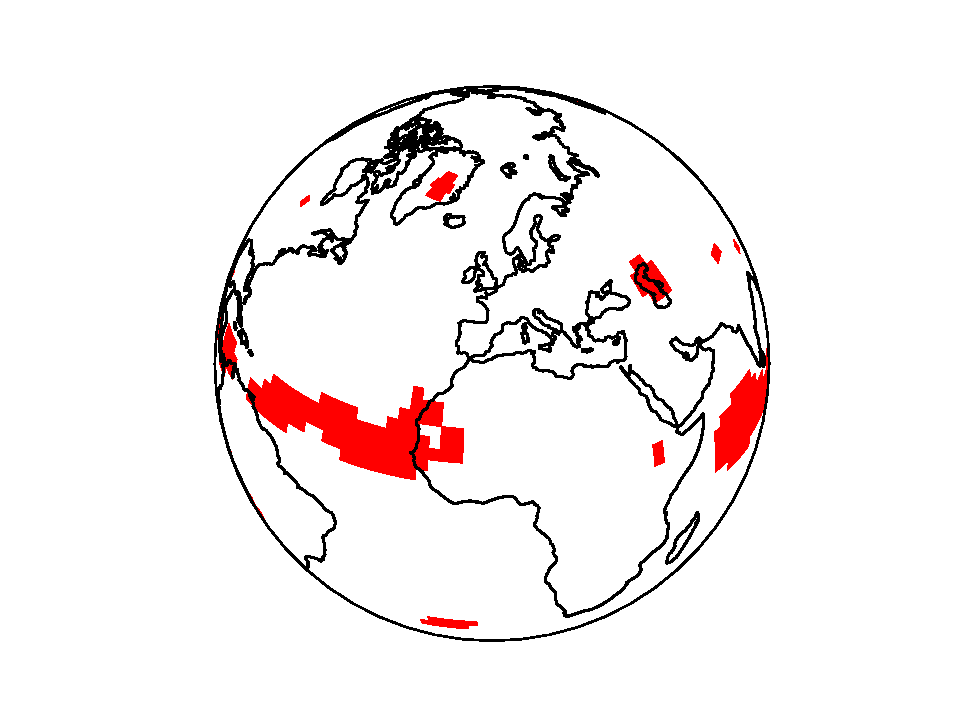
\includegraphics[scale=0.6]{sig-north.pdf}
    \caption{Northern hemisphere}
  \end{subfigure}%
  \begin{subfigure}{.6\paperwidth}
    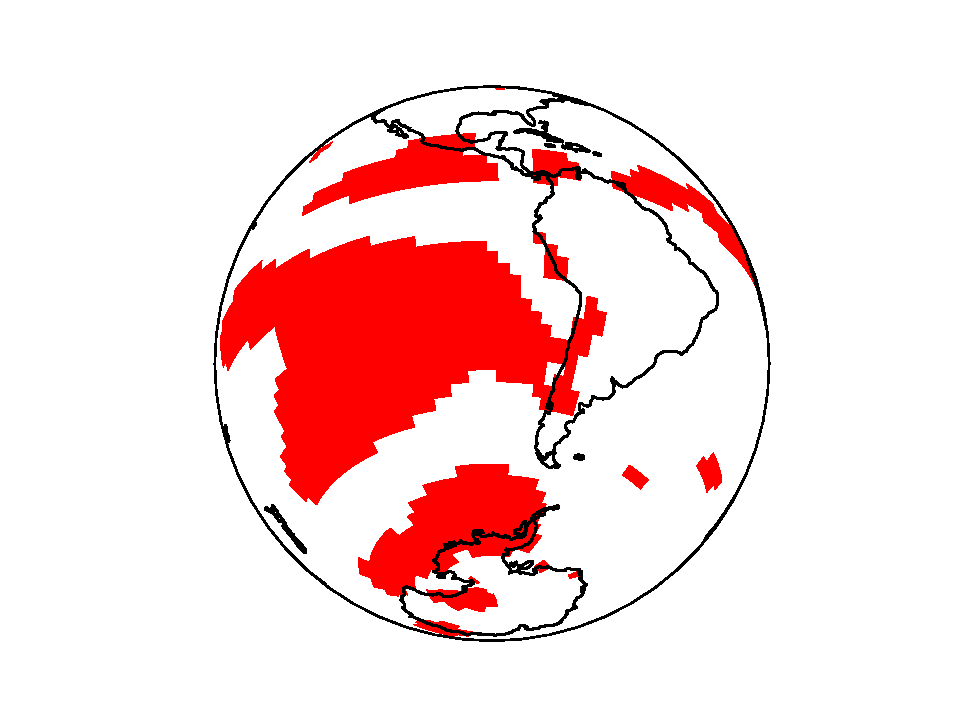
\includegraphics[scale=0.6]{sig-south.pdf}
    \caption{Southern hemisphere.}
  \end{subfigure}
  \caption{Significance at $\alpha = 0.01$}
  \label{fig:sig-global}
\end{figure}

Given that the data we have is mainly extrapolated from a limited set
of meteorological stations I do not think that we should conclude that
any significant changes have occurred. One can note that the changes
that we have identifies are larger over areas where we have the least
data (Pacific ocean, Antarctica). In all areas where we have more data
(Europe, North America) we see no changes at all. The two outliers
(Greenland, Caspian sea) might well be two stations that changed
location or equipment. I would not be comfortable to draw any
conclusions more than that changes over the period have been small.

\section*{Task II - correlation over time}

Even if we have no significant changes between the first and second
period we do of course have local changes during the whole period. The
question is if these local changes are correlated. One would of course
expect that we have a large positive correlation between adjacent grid
cells but the interesting question is if we have correlation, positive
or negative, between areas that are wide apart; for example an increase
of air pressure in one region is correlated in a decrease in another
region.

\begin{figure}[ht!]
  \centering
  \hspace*{-2cm}
  \begin{subfigure}{.5\paperwidth}
    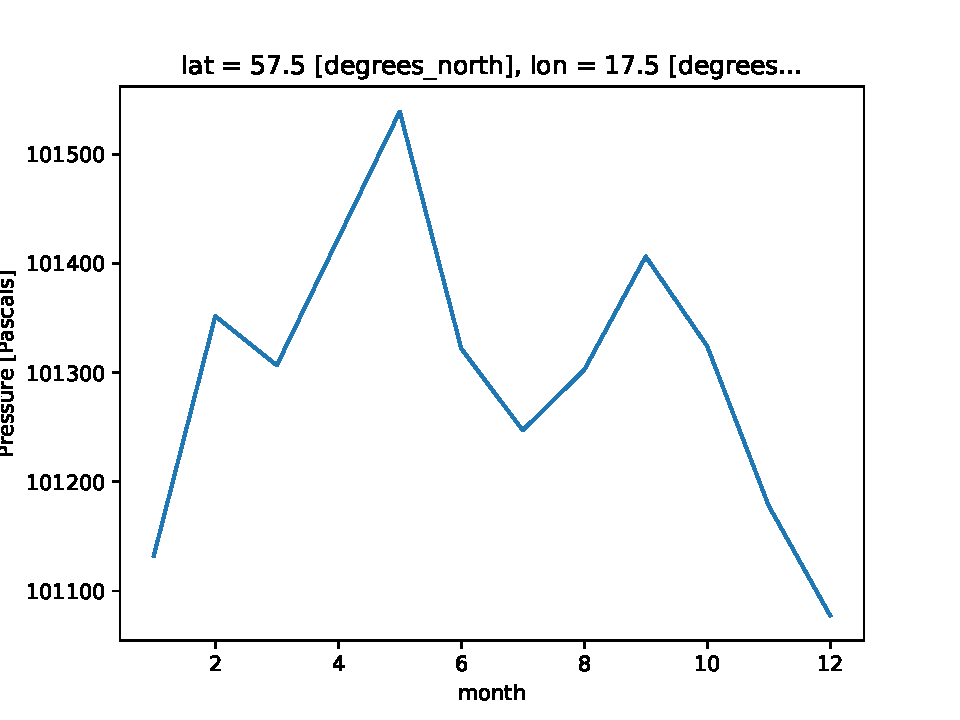
\includegraphics[scale=0.5]{stockholm-year.pdf}
    \caption{Yearly cycle.}
  \end{subfigure}%
  \begin{subfigure}{.5\paperwidth}
    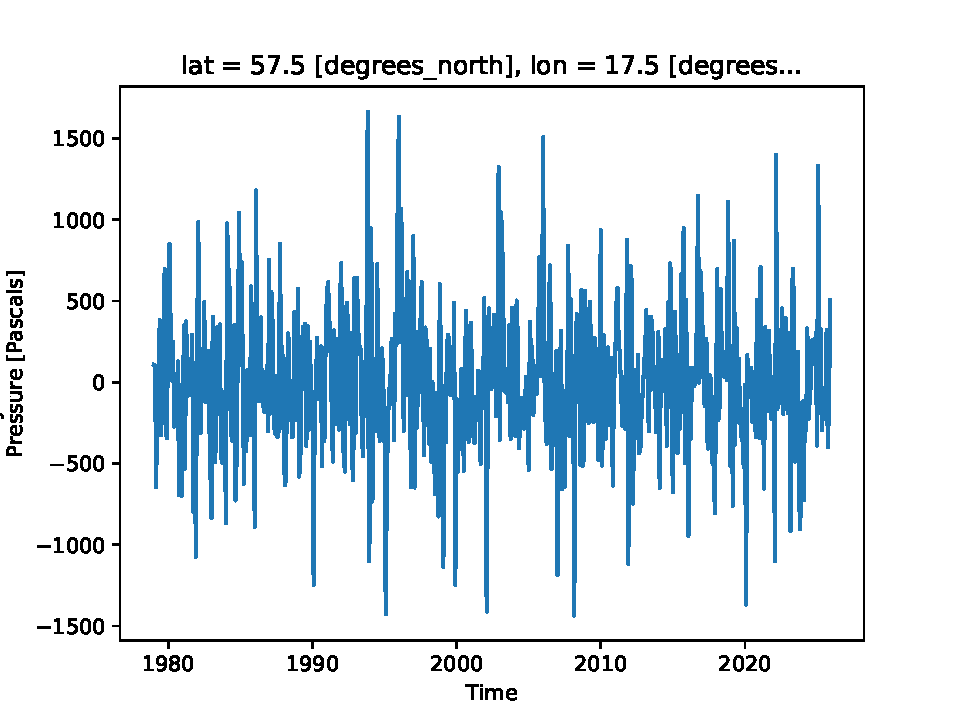
\includegraphics[scale=0.5]{stockholm-anom.pdf}
    \caption{Montly anomalies.}
  \end{subfigure}
  \caption{The grid covering Stockholm.}
  \label{fig:stockholm-anom}
\end{figure}

In order to better find these correlations we first remove any
seasonal pattern from the measurements. If we for example look at
Fig.\ref{fig:stockholm-anom} that shows the average monthly air
pressure over a year in Stockholm, we see that it varies over the
year. The winter months have in general a lower pressure and the
highest pressure is found during the spring months. If we now subtract
each monthly mean value from the measured values we obtain the
anomalies over the period that does not depend on the time of year. 

Our task is to look at the aggregated anomalies over the northern
hemisphere (north of $20\degree\; N$) during the winter months (Dec,
Jan, Feb). We start by selecting the interesting months but when we
average them we want the December record of one year be average
together with the January and February records of the next year. We
note that the first winter only contain January and February and the
last winter only the records from December so these are excluded in
the analysis.

When we examine the data over the northern hemisphere we should take
into account that the grids are of different sizes. A grid closer to
the poles is smaller compared to a grid close to the equator. If we
did not take this into account the cells closer to the north pole
would be over represented. To counter this we compute a weight matrix
where each grid gets a weight that is proportional to its size.

Since each grid is a cell with an north-south length that does not
vary but where the west-east length is proportional $cos(lat)$ we
compute a weight matrix with $\sqrt{cos(lat)}$. Choosing the square
root is justified by the fact that the analysis will square the
measurements so the computed weighted values will be weighted by $cos(lat)$. 

The result of running a EOF analysis is shown in
Fig. \ref{fig:eof}-a. We now see that we have an interesting areas of
anti-variability. There is a large area north-east of Island with
negative values and an area east of Azores with positive values. This
means that when we have higher pressure (than normal) over the Azores
we are more likely to find a lower (than normal) pressure over
Island. This is most certainly a sign of the North Atlantic Oscillation
(NOA).

\begin{figure}[ht!]
  \centering
  \hspace*{-3cm}
  \begin{subfigure}{.5\paperwidth}
  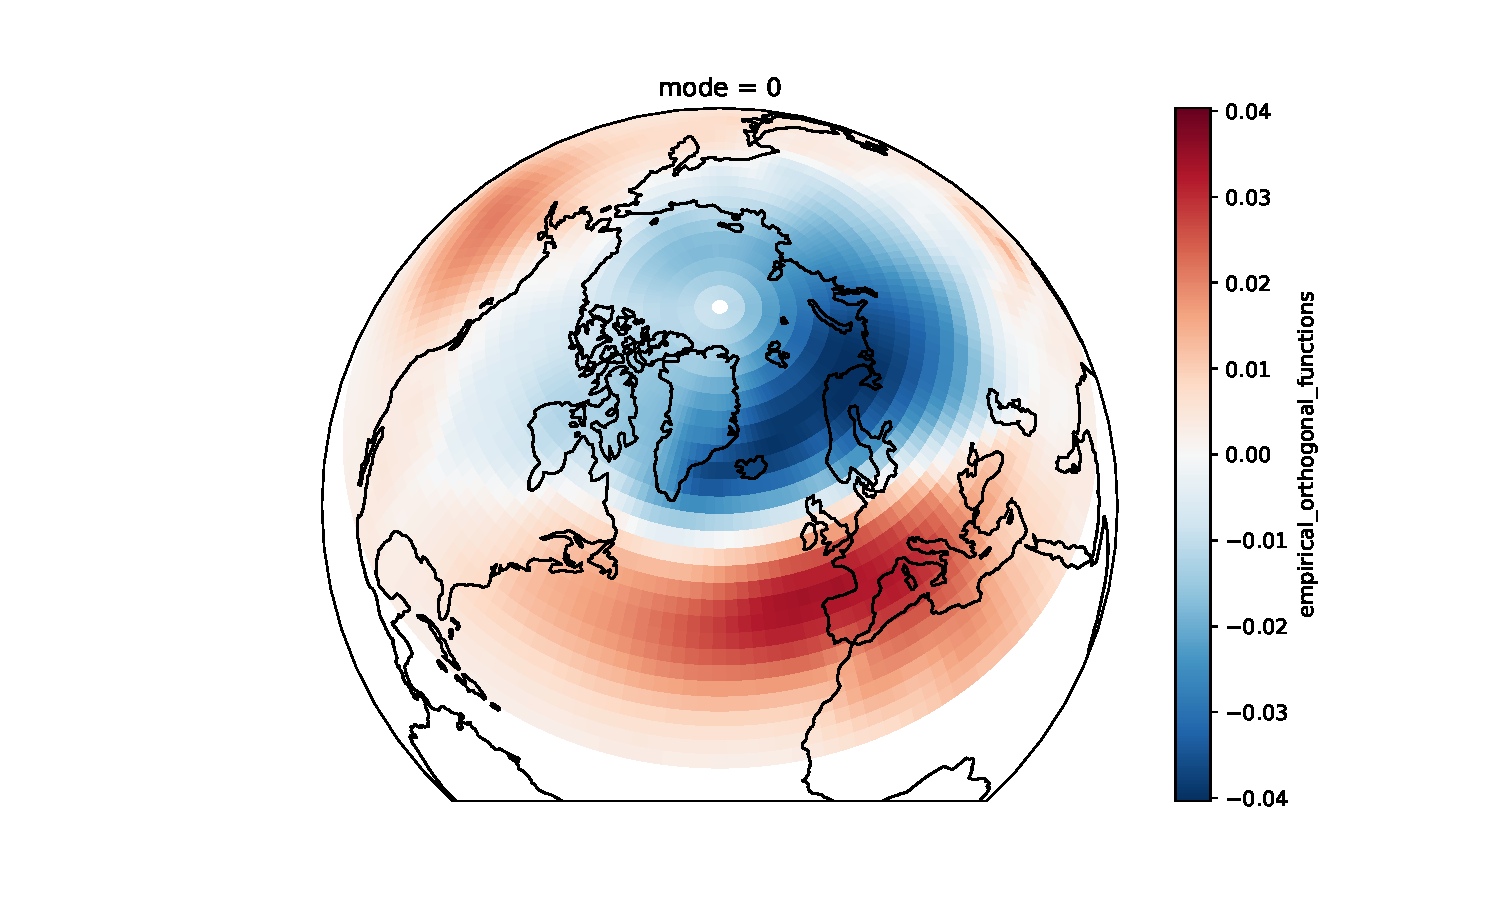
\includegraphics[scale=0.4]{winter-nh-eof.pdf}
  \caption{co-variability.}
  \end{subfigure}%
  \begin{subfigure}{.5\paperwidth}
    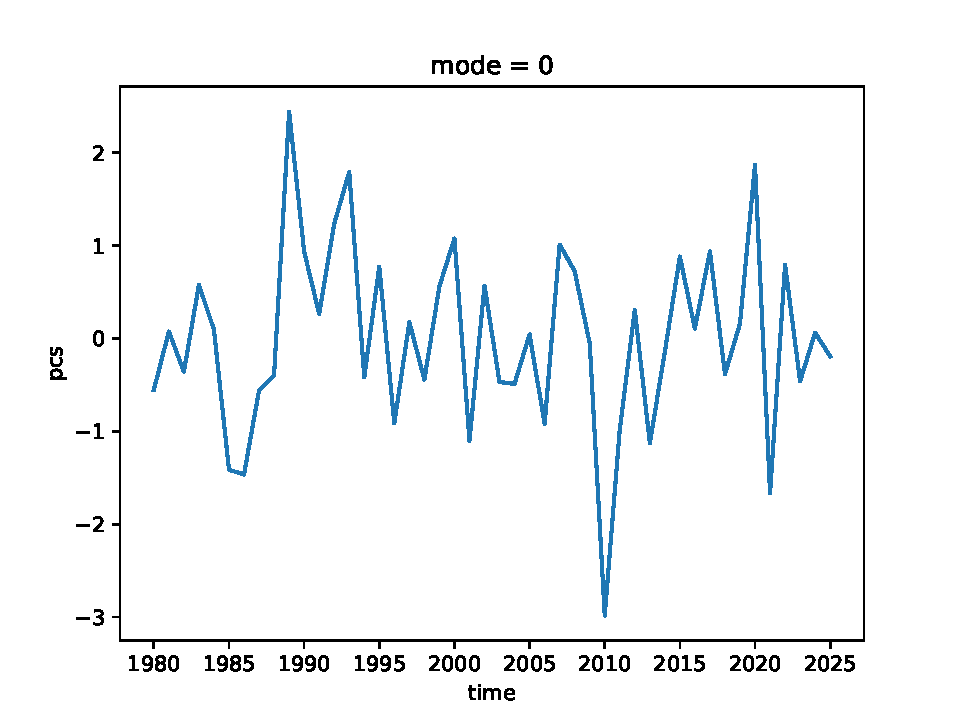
\includegraphics[scale=0.5]{winter-nh-pc1.pdf}
    \caption{principle component 1}
  \end{subfigure}
  \caption{Northern hemisphere: EOF analysis of the winter mean sea level pressure }
  \label{fig:eof}
\end{figure}

The interesting question now is what this oscillation looks like. If
we only know the co-variability we don't know if this variability is
on a yearly basis or on a five year basis. We need to look
at the {\em principle component 1} that was derived in the
analysis.

As seen in Fig. \ref{fig:eof}-b) there is no clear pattern of changes
in the principle component. We have a stronger relationship in 1989
and in 2020 and a strong negative relationship in 2010. If we do a
frequency analysis of the principle component we can use a regular
Fourier transform to obtain the dominating frequencies. As seen in
Fig.\ref{fig:freq}-a, there is a strong signal at approximately two
and a half year and another close to four years. There is also a
signal at around nine years and we should maybe not look further since
the total serie is only 46 years.

We could also use Welsh's method, which could remove some
noise. The result is shown in Fig.\ref{fig:freq}-b and we also here
see the signals at two and a half years, four years and now at close
to eight years. I'm currently not able to give any insight in the
difference nor which one to favor. A quick search on the NOA and
periodicity confirms that there should be a period of close to eight
years.

\begin{figure}[ht!]
  \hspace*{-4cm}
  \centering
  \begin{subfigure}{.5\paperwidth}
    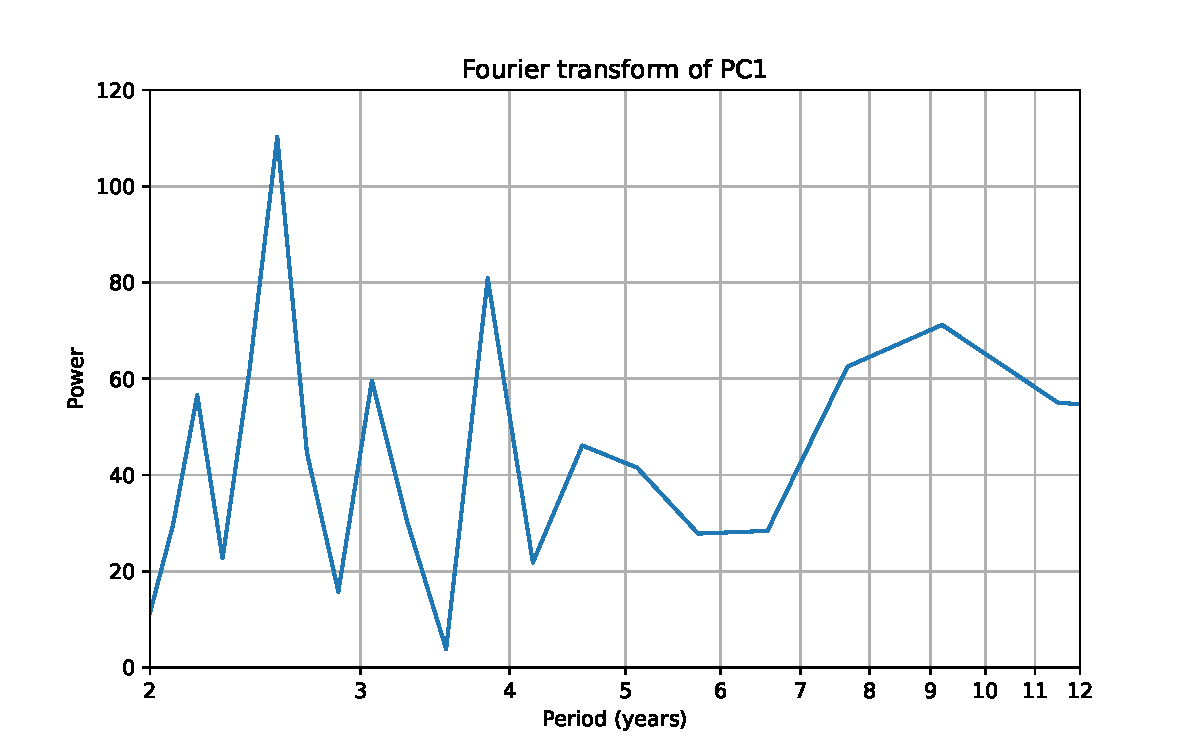
\includegraphics[scale=0.5]{pc1-fourier.pdf}
    \caption{Fourier transformation.}
  \end{subfigure}%
  \begin{subfigure}{.5\paperwidth}
    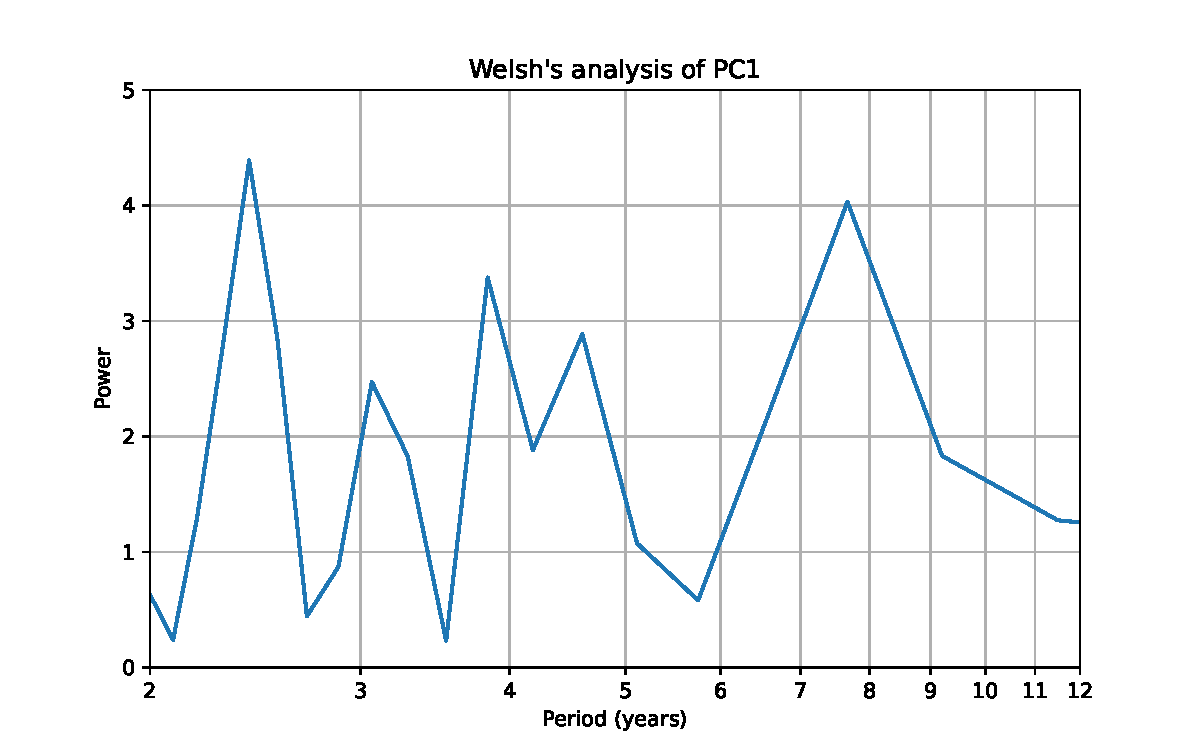
\includegraphics[scale=0.5]{pc1-welsh.pdf}
    \caption{Welsh's method}
  \end{subfigure}
  \caption{Northern hemisphere: frequency analysis of principle component 1.}
  \label{fig:freq}
\end{figure}

\section{Task III - Darwin vs Tahiti}

Our third task is to examine the spectrum of variability between the
area around Darwin (AUS) and Tahiti.  We select the nine grid cells
that are closest to either location and average the values of these
grids in two time series. For each serie we compute the anomalies by
subtracting the mean over the whole period.

{\em In my first try I also divided by the std but this had some
  unforseen consequences. The over all picture did not change but the
  regression analysis did not work as expected; there was no
  difference between having Darwin as predictor vs predicted.}

\subsection*{EOF analyisis}

Given the two series we can do an EOF analysis which give us the
values shown in Tab.\ref{tab:darwin-tahiti-eof}.

\begin{table}[ht!]
\centering
\begin{tabular}{ c c c }
 \textbf{EOF} & \textbf{ Darwin} & \textbf{ Tahiti} \\
\hline\\
%[-0.744886  ,  0.66719174],
%[-0.66719174, -0.744886  ]]

EOF1 & -0.74 & 0.67\\
EOF2 & -0.67 & -0.74\\
\end{tabular}
\caption{EOF of Darwin vs Tahiti}
\label{tab:darwin-tahiti-eof}
\end{table}

The EOF numbers indicate that the two series are out of phase (different sign in
EOF1). Since we only have two series we can also look at a scatter-plot
as shown in Fig.\ref{fig:darwin-tahiti}-a the negative correlation is
visible but not very strong (-0.4). In Fig. \ref{fig:darwin-tahiti}-b
that shows a 12-month running mean, we clearly see how the time series
are out of phase.

\begin{figure}[ht!]
  \hspace*{-4cm}
  \centering
  \begin{subfigure}{.5\paperwidth}
  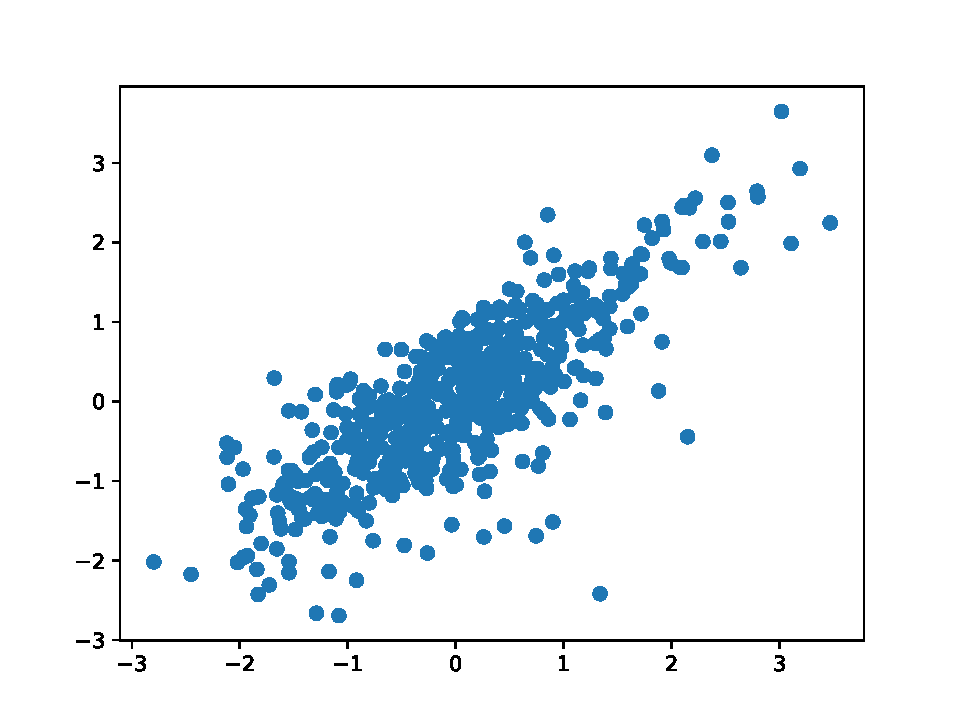
\includegraphics[scale=0.5]{darwin-tahiti-scatter.pdf}
  \caption{Scatter plot.}
  \end{subfigure}%
  \begin{subfigure}{.5\paperwidth}
    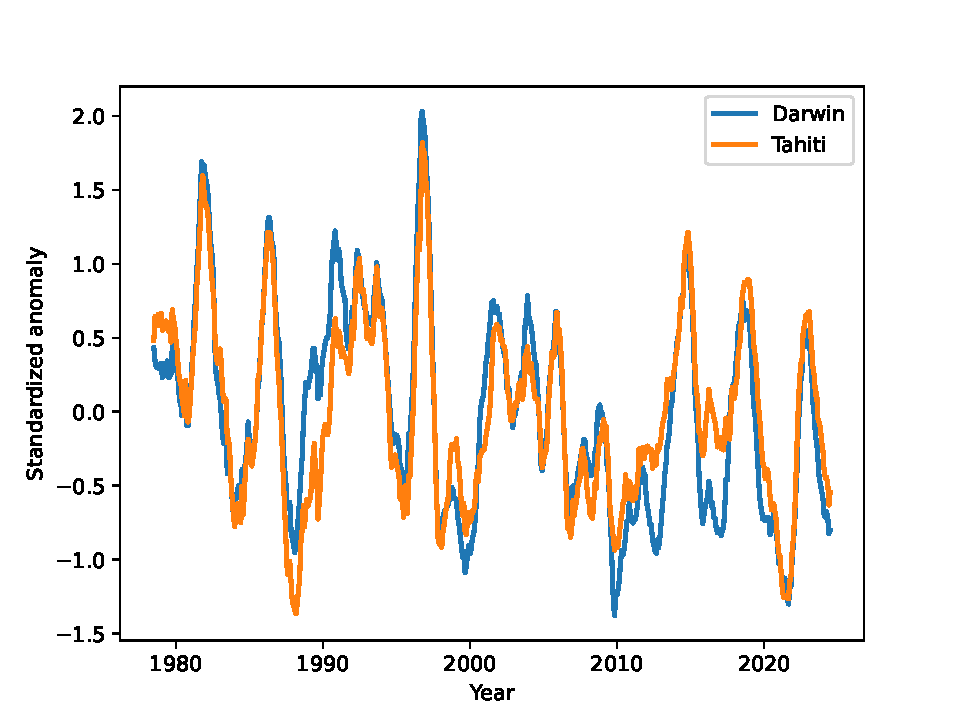
\includegraphics[scale=0.5]{darwin-tahiti-running.pdf}
    \caption{12-month running mean}
  \end{subfigure}
  \caption{Darwin-Tahiti: anomaly of mean sea level pressure.}
  \label{fig:darwin-tahiti}
\end{figure}

If we investigate {\em principle component 1}, we can do a fourier
transformation and see if we can find any perodicity. In
Fig. \ref{fig:darwin-tahiti-fourier} we see that we have periodicity
at 2 to 3 years, 4 and 12 years. The 2 to 3 and 4 year periods
correspond to the El Niño Southern Oscillation (ENSO). The 12 year
cycle should be taken with a grain of salt since we only have
fortyseven years of data to start with i.e. less than four periods.

\begin{figure}[ht!]
  \centering
  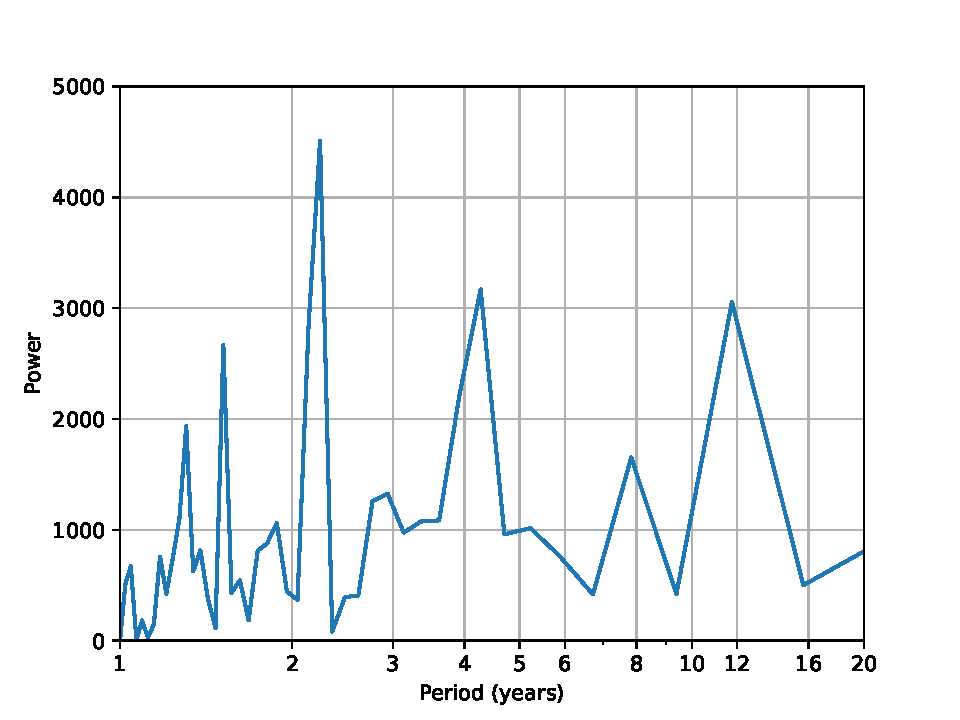
\includegraphics[width=0.4\paperwidth]{darwin-tahiti-pc1.pdf}
  \caption{Darwin-Tahiti: PC1, Fourier transformation.}
  \label{fig:darwin-tahiti-fourier}
\end{figure}

\subsection*{Darwin - Tahiti}

If we take our Darwin and Tahiti time series we can correlate them to
all time series around the globe; the result is shown in
Fig. \ref{fig:darwin-tahiti-pacific}. It is clear that we have two
large areas that are correlated to the Darwin and Tahiti series.  The
cycles that determine the difference between Darwin and Tahiti is well
correlated with changeds in a region between the Indian Ocean and South America.

\begin{figure}[ht!]
  \hspace*{-4cm}
  \centering
  \begin{subfigure}{.5\paperwidth}
  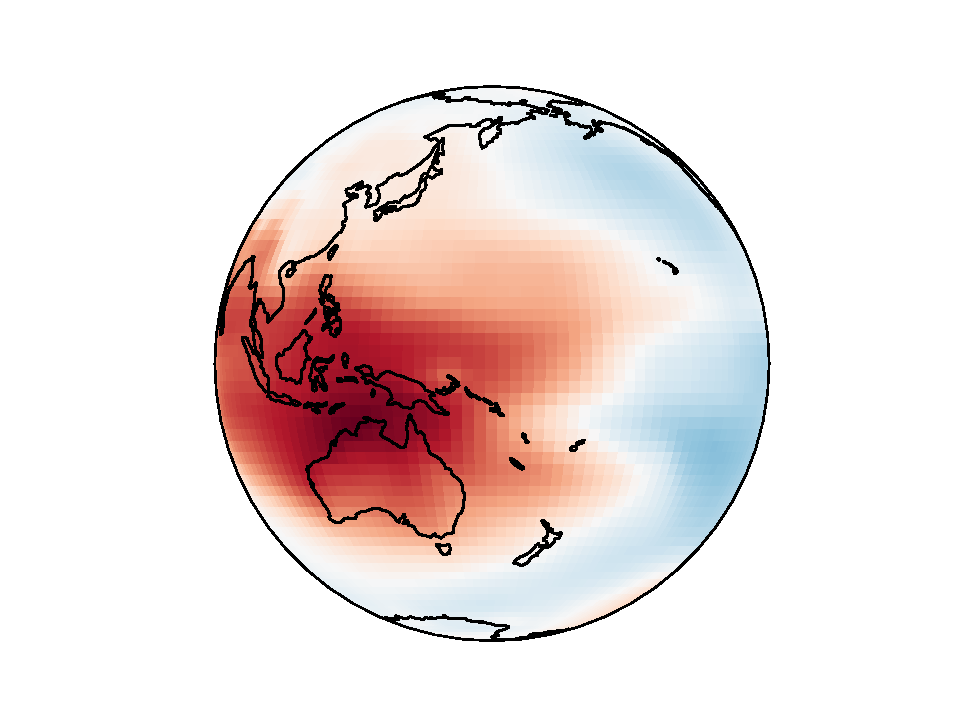
\includegraphics[scale=0.5]{darwin-pacific.pdf}
  \caption{Correlation with Darwin}
  \end{subfigure}%
  \begin{subfigure}{.5\paperwidth}
    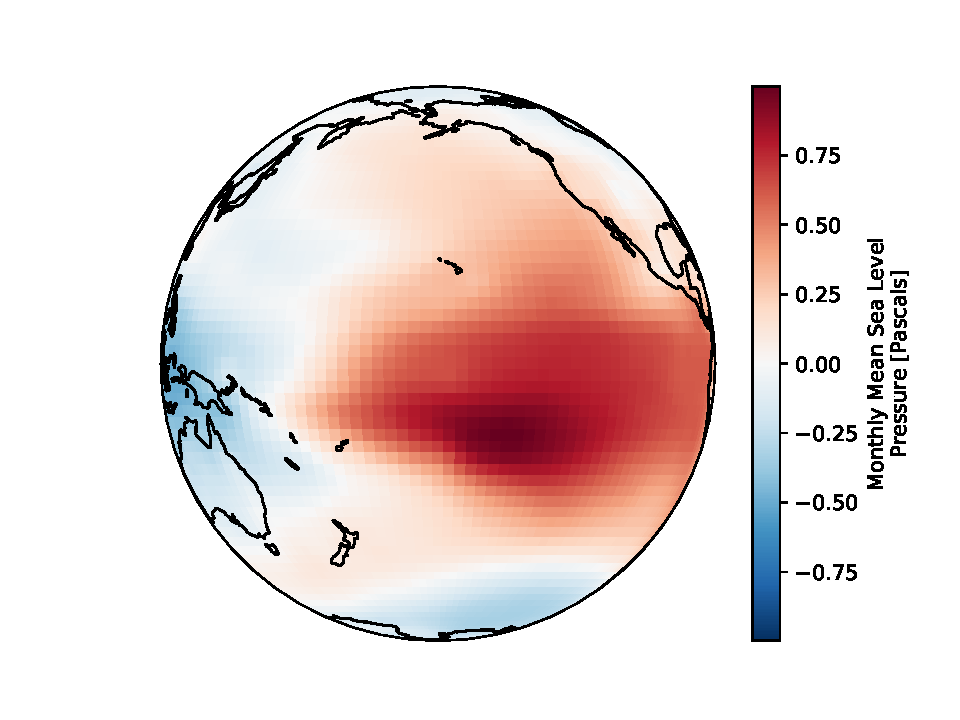
\includegraphics[scale=0.5]{tahiti-pacific.pdf}
    \caption{Correlation with Tahiti}
  \end{subfigure}
  \caption{Correlation with Darwin and Tahiti.}
  \label{fig:darwin-tahiti-pacific}
\end{figure}

If we look at the other side of the globe we see that the correlation
with air pressure anomalies is very weak in general and over Europe it
is non-existing. Note that we are looking at the El Niño fenomena and
there might be other climatologies (cloudiness, rain, temperature,
...) that are affected.

\begin{figure}[ht!]
  \hspace*{-4cm}
  \centering
  \begin{subfigure}{.5\paperwidth}
  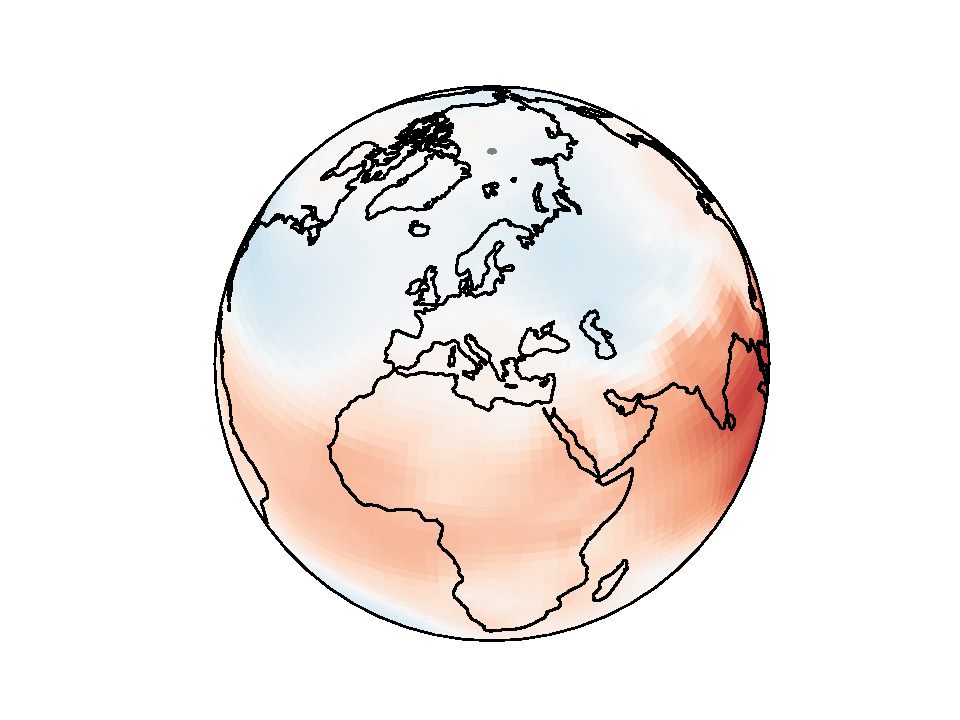
\includegraphics[scale=0.5]{darwin-europe.pdf}
  \caption{Correlation with Darwin}
  \end{subfigure}%
  \begin{subfigure}{.5\paperwidth}
    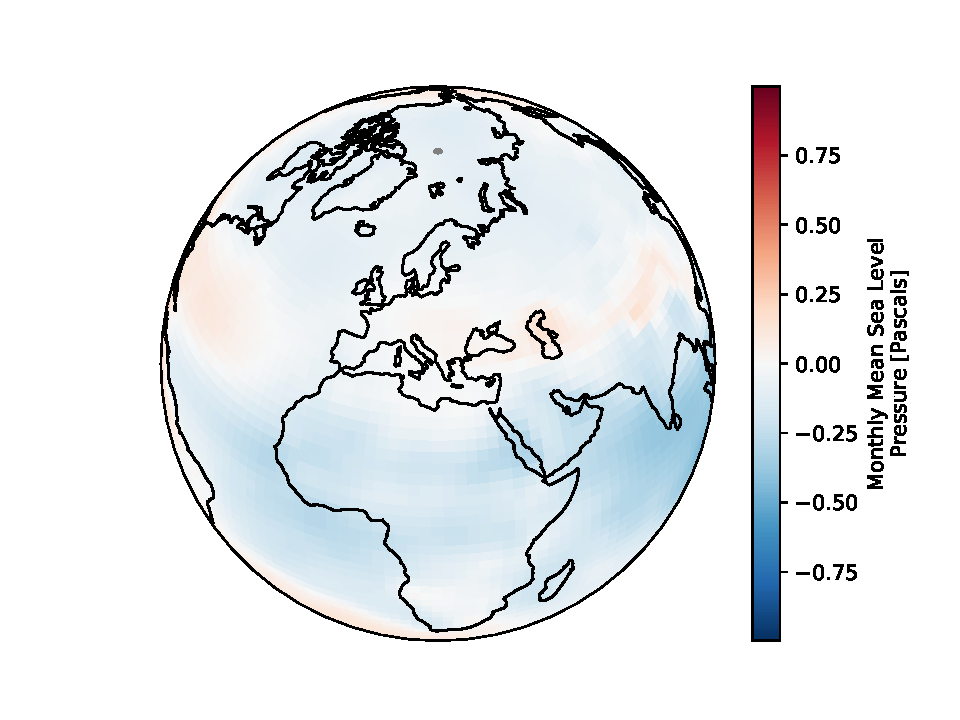
\includegraphics[scale=0.5]{tahiti-europe.pdf}
    \caption{Correlation with Tahiti}
  \end{subfigure}
  \caption{Correlation with Darwin and Tahiti.}
  \label{fig:darwin-tahiti-europe}
\end{figure}

\subsection*{Darwin regression analysis}

If we look at the data we have from our Darwin location, we have
determined that is is well correlated with cells in the Indian Ocean
and south-east part of the Pacific. We can now pose the question if
the air pressure at Darwin is a {\em predictor} or a {\em
  predictand}. An indication is gained by doing a regression analysis
for each cell and see how well they either predict or is predicted by
the Darwin serie.

For each grid cell we first do a regression analysis for:
$$ {\rm cell}(t) = m + k\times {\rm darwin}(t) $$

and determine $k$. We then have a map of how strongly a grid cell is
depending on the Darwin time serie. We then do the opposite and do a
regression analysis over:

$${\rm darwin}(t) = m + k\times {\rm cell}(t)$$

The two analysis show some difference. In Fig.\ref{fig:darwin-india}-a
we see that Darwin can be used as a predictor for the equatorial area
from the Indian Ocean to the pacific. The higest predictable factor is
the area of Indonesia. If we look at Fig.\ref{fig:darwin-india}-b we
se that the region that serves as the best predictor is the Australian
continent. 

\begin{figure}[ht!]
  \hspace*{-4cm}
  \centering
  \begin{subfigure}{.4\paperwidth}
    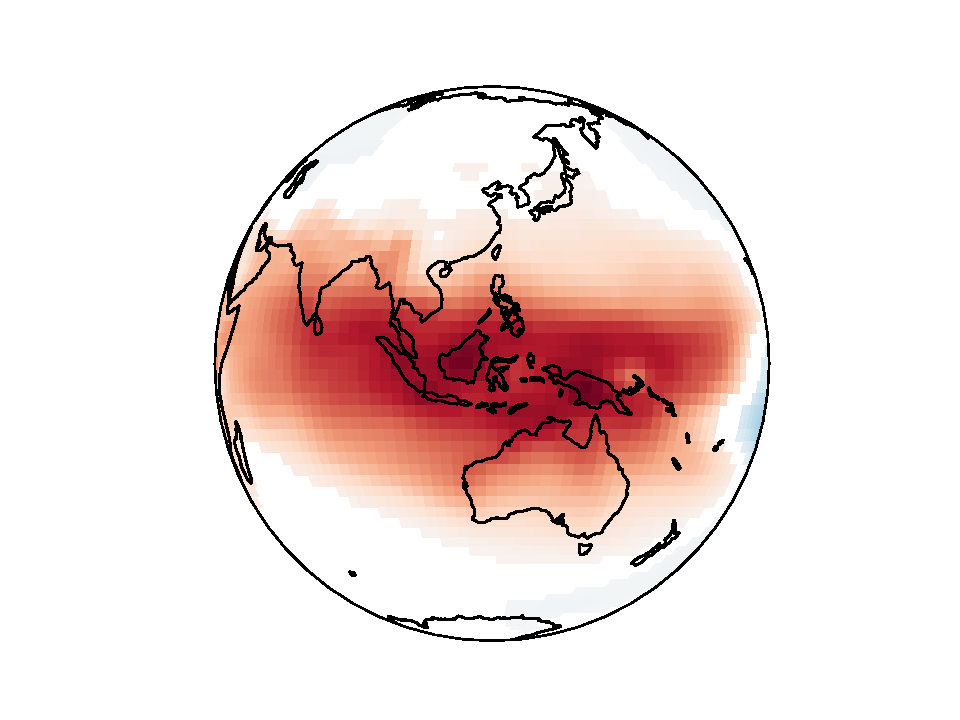
\includegraphics[scale=0.5]{darwin-predictor-india.pdf}
    \caption{Darwin as predictor.}    
  \end{subfigure}%
  \begin{subfigure}{.6\paperwidth}
    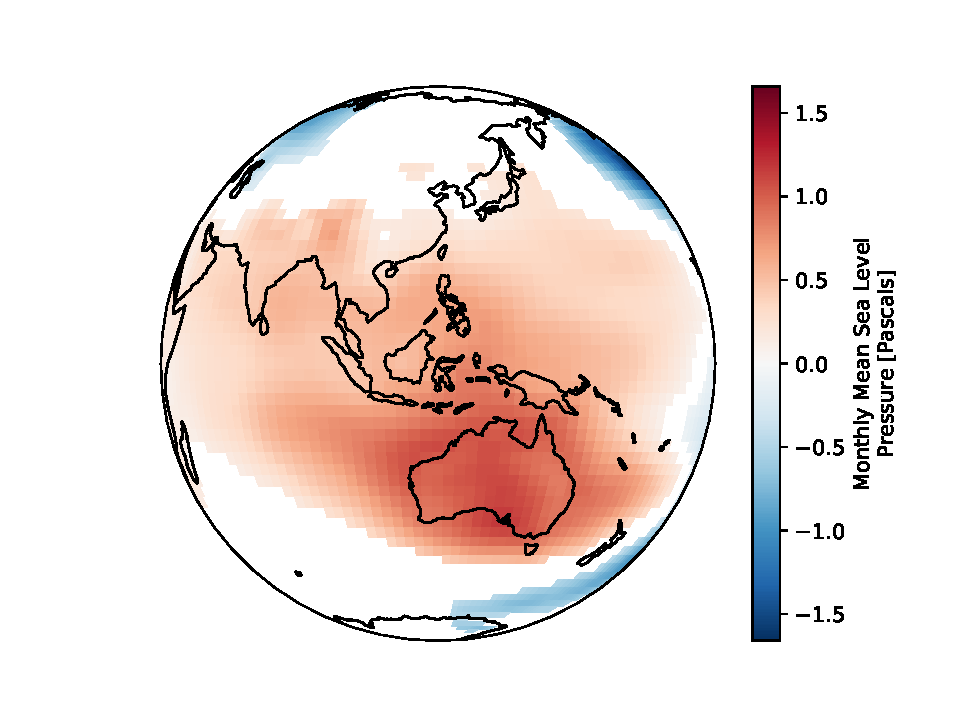
\includegraphics[scale=0.5]{darwin-predictand-india.pdf}
    \caption{Darwin as predictand.}
  \end{subfigure}

  \caption{Darwin: regression analysis Indian Ocean.}
  \label{fig:darwin-india}
\end{figure}

If we look at the globe from the other side we see less of an
influence in either direction. Yes we have some negative predictors in
the south Pacific and this is of course related to the same out of
phase correlation between Darwin and Tahiti that we saw earlier.

We have one area in the Pacific just north of Antarctica that
according to these number could serve as a strong predictor of the air
pressure in Darwin. This is somewhat surprising especially since the
reverse does not hold - the air pressure in Darwin does not serve as a
good predictor for the Antarctic region. This could be an effect of
difference in variance between the two areas. If we have small
anomlies in the Antarctic reagion, but correlated, these must be
scaled with a higher factor. The reverse also holds, a large
difference in Darwin must be scaled down.



\begin{figure}[ht!]
  \hspace*{-4cm}
  \centering
  \begin{subfigure}{.4\paperwidth}
    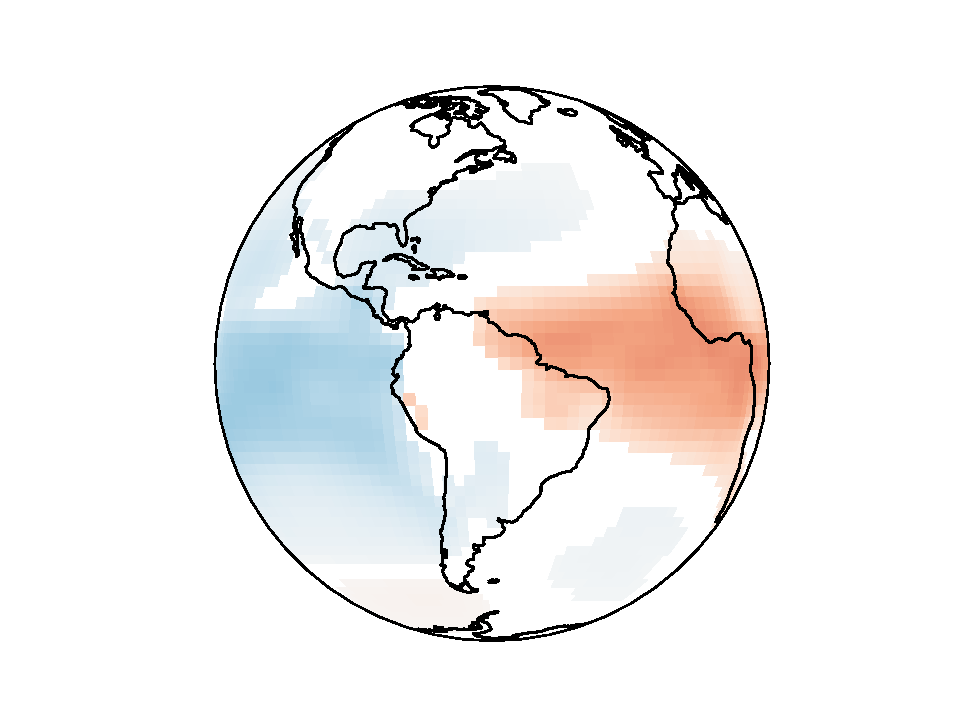
\includegraphics[scale=0.5]{darwin-predictor-atlantic.pdf}
    \caption{Darwin as a predictor.}
  \end{subfigure}%
  \begin{subfigure}{.6\paperwidth}
    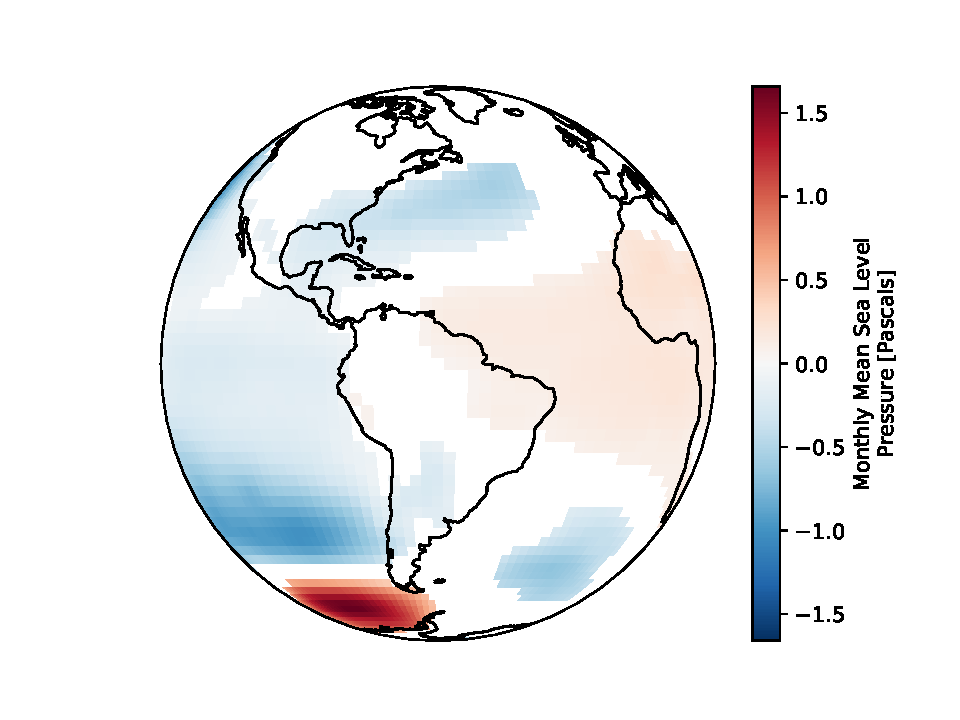
\includegraphics[scale=0.5]{darwin-predictand-atlantic.pdf}
    \caption{Darwin as a predictand.}
  \end{subfigure}

  \caption{Darwin: regression analysis South Atlantic}
  \label{fig:darwin-atlantic}

\end{figure}


\section*{Task VIa - clustering}



The last task is looking at the mean sea level pressure in the
northern hemispher again. This time we take all the time series and
first calculate their anomalies. Then we treat each time as a multi
dimensional vector (one dimension per grid) and try to identify the
clusters in this space.

\subsection*{k-means clustering}

To our help we have the {\tt scikit-learn} package that implements a
set of machine leraning techniques. We use {\tt sklearn.cluster} and
search for a solution with two clusters. In figure
Fig.\ref{fig:nh-cluster} we se the center images of these two clusters. We
can interpret this as two separate states that the air preassure on
the northern hemisphere find favorable.

The two states have high and low pressures over more or less that same
areas. In the first state we have higher than average pressure
north-west of Greenland while lower than normal pressures in the north
Atlantic and over Europe. In the second state the conditions are
reversed. 

\begin{figure}[ht!]
  \hspace*{-4cm}
  \centering
  \begin{subfigure}{.4\paperwidth}
  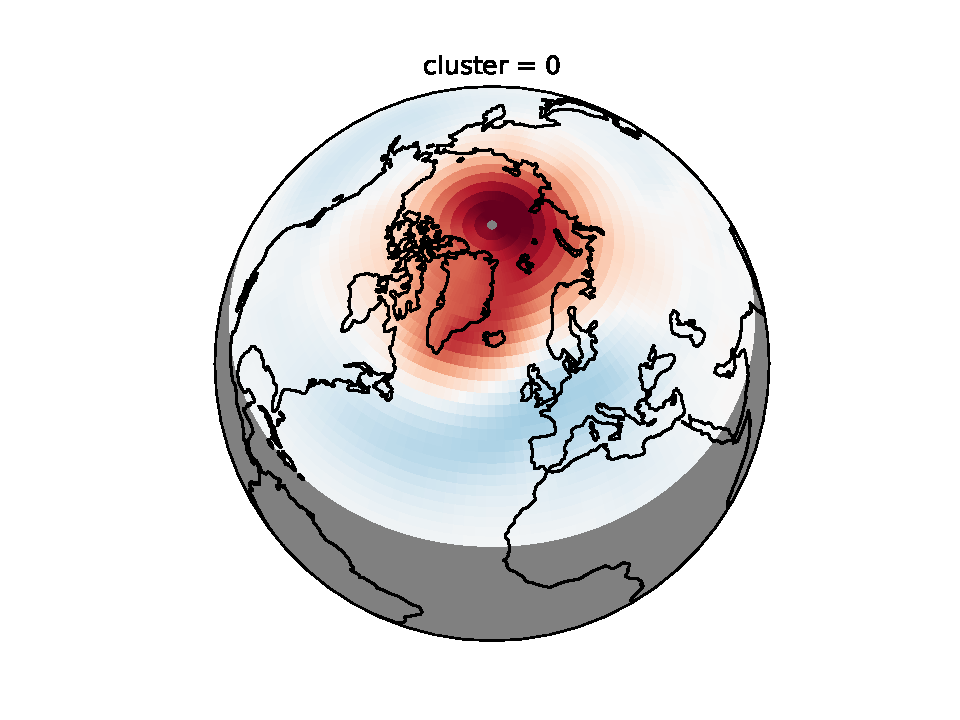
\includegraphics[scale=0.6]{nh-cluster0.pdf}
  \caption{Cluster 0 .}
  \end{subfigure}%
  \begin{subfigure}{.6\paperwidth}
    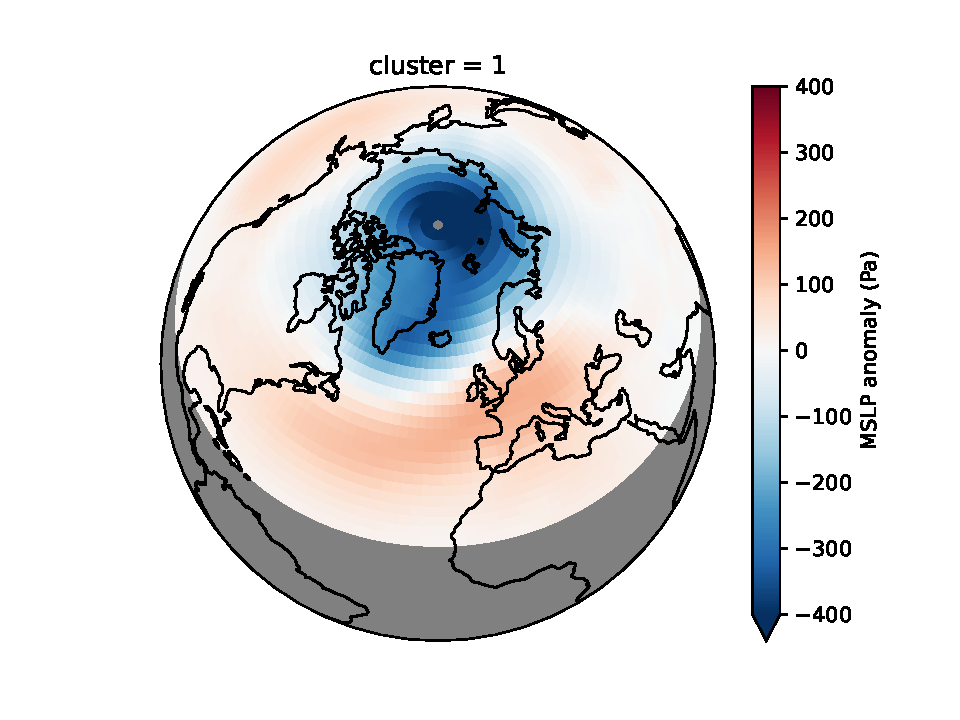
\includegraphics[scale=0.6]{nh-cluster1.pdf}
    \caption{Cluster 1}
  \end{subfigure}
  \caption{Norther hemipshere clustering of montly mean sea level pressure.}
  \label{fig:nh-cluster}
\end{figure}

\subsection*{Hierarchical clustering}

An alternative way to perform clustering is to do an hierarchical
clustering. This means that we start from all individual maps and
group the two maps that are most similar. Repeating this process will
create larger and larger clusters until we are left with two
clusters. The two clusters represent $295$ and $269$ months so the months
are more or less equally divided in the clusters.

Not knowing too much about different hierarchical methods we use {\tt
  linkage()} in the {\tt scipy.cluster.hierarchy} module. This will
give us a {\em dendrogram} with the clusters shown in
Fig.\ref{fig:dendrogram}. It is not immediately visible in the plot
how large the clusters are but if we add up the clusters under the
first cluster we get $124$ months while the second cluster consists of
$440$ months. The second cluster is then divided into two sub clusters
of sizes $122$ and $318$ months; this is clearly different from the
k-means clustering..

\begin{figure}[ht!]
  \centering
  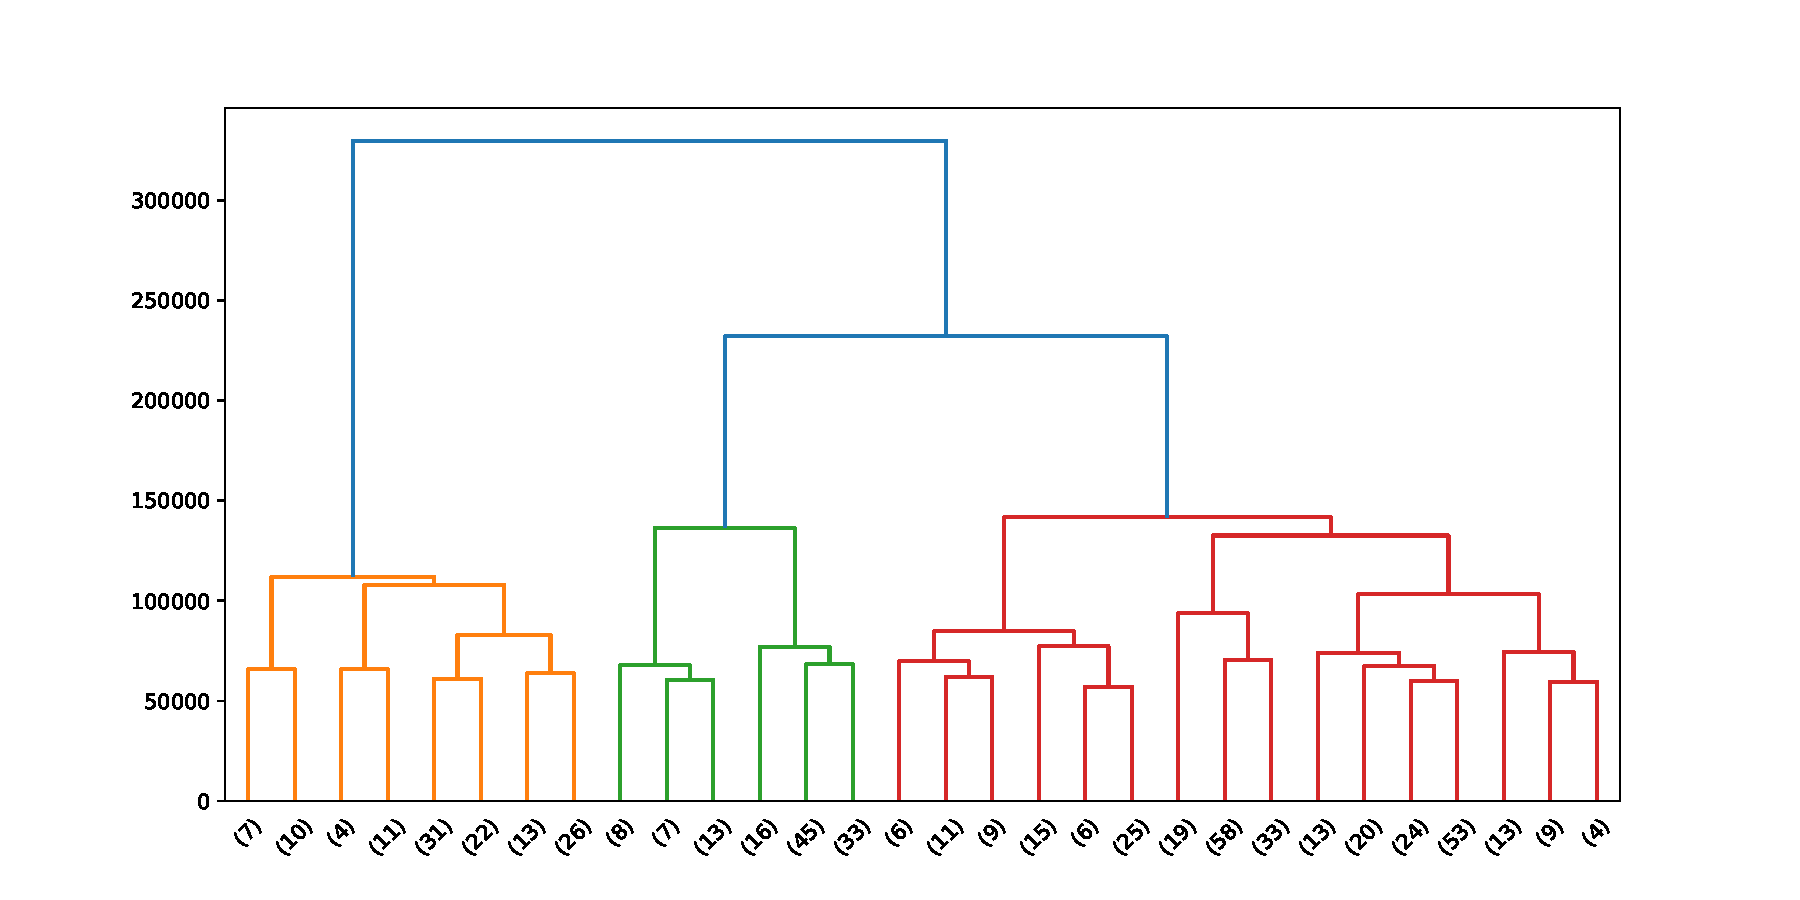
\includegraphics[width=0.4\paperwidth]{dendrogram.pdf}
  \caption{Northern hemisphere: dendogram of hireacical clustering.}
  \label{fig:dendrogram}
\end{figure}

We can generate two maps that correspond to the two clusters as shown
in Fig.\ref{fig:nh-hierarchical}. These maps should be compared to the
ones obtained by the k-means clustering shown in
Fig.\ref{fig:nh-cluster}. As seen the images are similar but the
hierarchical method has the anomalies in the first cluster larger
compared to the k-means version; the opposit is true for the second
cluster. This could be an effect of how which months are inclused in
each cluster; having only $122$ months in the first cluster would of
course mean that we have a stringer signal compared to a cluster with
$440$ months.


\begin{figure}[ht!]
  \hspace*{-4cm}
  \centering
  \begin{subfigure}{.4\paperwidth}
  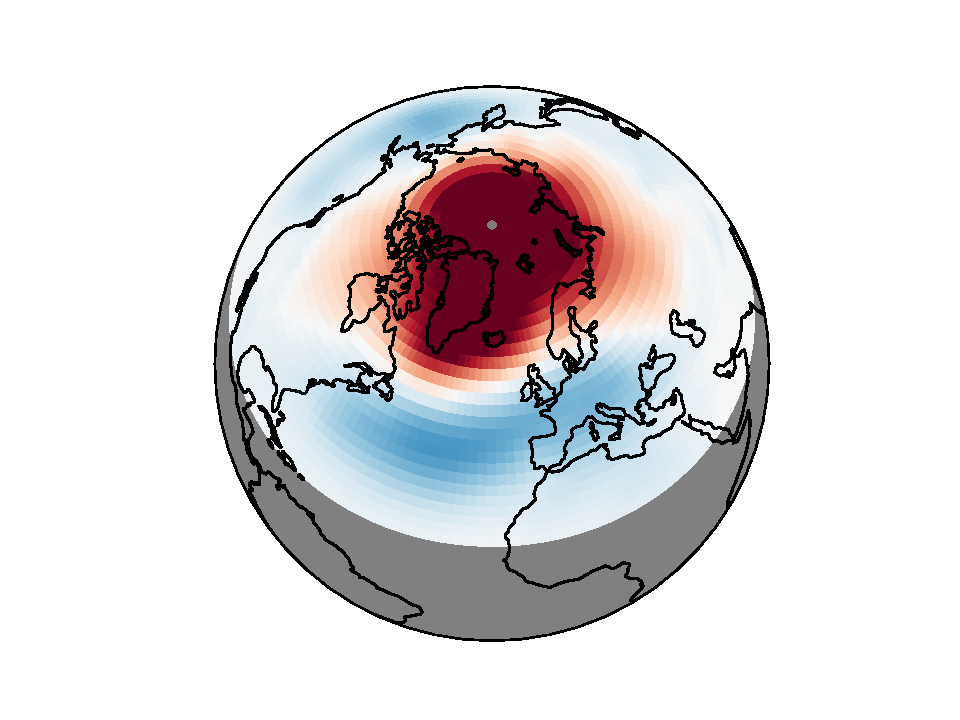
\includegraphics[scale=0.6]{nh-hierarchical0.pdf}
  \caption{Cluster 0 .}
  \end{subfigure}%
  \begin{subfigure}{.6\paperwidth}
    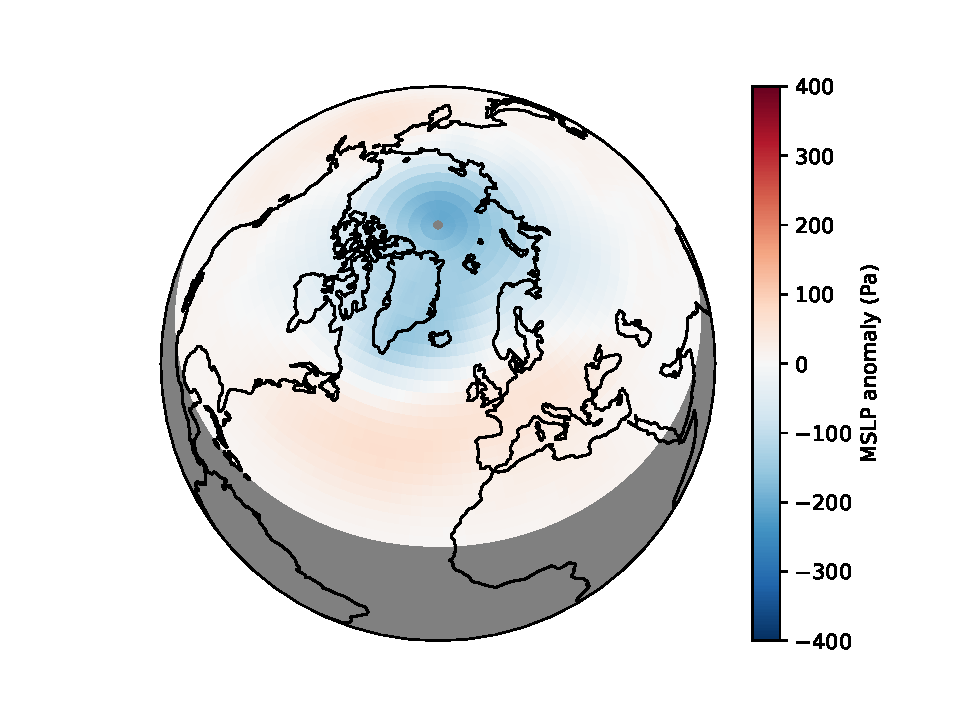
\includegraphics[scale=0.6]{nh-hierarchical1.pdf}
    \caption{Cluster 1}
  \end{subfigure}
  \caption{Norther hemipshere: hierarchical clustering.}
  \label{fig:nh-hierarchical}
\end{figure}

\section*{Summary}

An interesting exercise that for sure did take time. Allthough an
experienced programmer this is only the second time I've used Jupyter
and Python for a project. This is the first time I've used OpenAI:s
ChatGPT for programming and I would not have been able to complete the
project in time if I only had the manuals to work with.

The statistical packages used are of course to great help when looking
at the data. Doing even the simplest transformation by hand would be a
tedious task. That said it aslso hides what is actually done and it's
very easy to use a method, for example Welsh's method, without having
a clue of what is actually done.

The plotting tools are also wounderful and gives you a far better
understanding of what is happening when we are working with global
data. If I would have to use my regular skills in displaying data in
graphs much understanding would be lost. It is of course also a danger
twht "an image sais more than a thousand words" but one does not
really understand what is shown.

\end{document}
